\documentclass{article}
\usepackage{ucs}
\usepackage[utf8]{inputenc}

\title{Algoritmo UCB}
\author{Nelson Steven Sanabio Maldonado}
\date{Junio 2018}

\usepackage{natbib}
\usepackage{graphicx}
\usepackage{amsmath}
\usepackage{mathtools}
\usepackage{amssymb}
\usepackage{parskip}



\begin{document}

\maketitle

\section{Algoritmo}
La mecánica del algoritmo de confianza superior (UCB) es
simple. En cada ronda, simplemente tiramos del brazo que
tiene la estimaci\'on de recompensa emp\'irica m\'as alta
hasta ese punto m\'as un t\'ermino que es inversamente
proporcional al n\'umero de veces que se ha jugado el brazo.
M\'as formalmente, defina ni, t como el n\'umero de veces
que se ha jugado el brazo $i$ hasta el momento $t$.
Defina $rt \in [0, 1]$ ser la recompensa que observamos en el momento $t$. Define $I_t \in \{1. . . N\}$ para ser la elección del brazo en el tiempo $t$. Entonces la estimación de recompensa empírica del brazo $i$ en el tiempo $t$ es:
$$\mu_{i,t} = \frac{\sum_{s=0\colon I_s=i}^{t}r_s }{n_{i,t}}$$
UCB asigna el siguiente valor a cada brazo $i$ en cada momento $t$:$$UCB_{i,t} := \mu_{i,t} + \sqrt{\frac{ln\>t }{n_{i,t}}}$$
El algoritmo UCB se da a continuación:
$$ 
\framebox{
\begin{minipage}[b][1.2\height]%
[t]{0.75\textwidth} \textbf{UCB}\\\\
\textbf{Input}: $N$ brazos, número de rondas $T\geq N$\\
\begin{enumerate}
    \item Para $t=1 ... N$, jugar brazo $t$\\
    \item Para $t = N+1 ... T, juego de brazo$
\end{enumerate}\\\\

$$I_t = arg_{i \in \{1...N\} } \max UCB_{i,t-1}$$
\end{minipage}
}
$$
Tenga en cuenta que estamos asumiendo (al menos en esta formulación) que jugaremos al menos N veces. Además, estamos actualizando implícitamente nuestra estimación empírica (1) cada vez que jugamos un brazo. Observe que en el tiempo $t$, el algoritmo utiliza el UCBi, $t-1$, que se puede calcular utilizando observaciones realizadas hasta el tiempo $t - 1$.




\begin{figure}[h!]
\centering
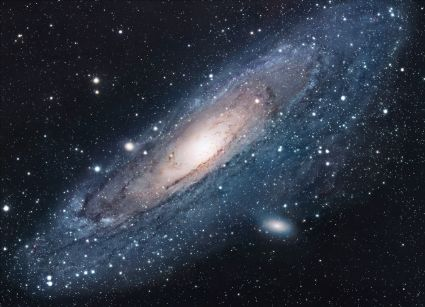
\includegraphics[scale=1.7]{universe}
\caption{The Universe}
\label{fig:universe}
\end{figure}

\section{Conclusion}
``I always thought something was fundamentally wrong with the universe'' \citep{adams1995hitchhiker}

\bibliographystyle{plain}
\bibliography{references}
\end{document}
